\documentclass{beamer}
\title[Footnote Title \hspace{2em}\insertframenumber/\inserttotalframenumber]{Main Title} %Note: Professor Groth is not a fan of slide numbering.
\subtitle{Sub-Title}
\author{A. Author}
\date{December 18, 2014}
\usetheme{Warsaw}
\usepackage[version=3]{mhchem}
\usepackage{caption}
\begin{document}

\addtocounter{framenumber}{-1}

\frame{\titlepage}

\begin{frame}
\frametitle{Frametitle}

{\color{blue} Colourful Sub-Title}
\begin{itemize}
\item First bullet level.
\begin{itemize}
\item Second bullet level.
\begin{itemize}
\item Third bullet level.
\end{itemize}
\end{itemize}
\item First bullet level again.
\end{itemize} 

\end{frame}

\begin{frame}
\frametitle{Frame With Figure}

\begin{figure}[h!]
\centering
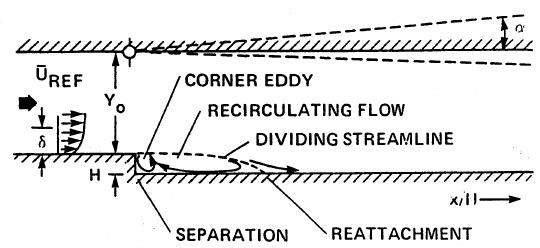
\includegraphics[width=0.5\textwidth]{./figs/BFS_FLOW_DRIVER.jpg}
\caption*{\tiny Typical Backward Facing Step Flow Configuration as an Example [Driver 1985]}
\end{figure}

\begin{itemize}
 \item Important bullet point.
\end{itemize} 
\end{frame}

\begin{frame}
\frametitle{Frame With Table}

\begin{itemize}
\item Important bullet point.
\end{itemize}

\begin{tiny}
\begin{table}[t!]
\begin{center}
\caption*{{\tiny Re-Attachment Lengths Predicted by DES Turbulence Models}}
\begin{tabular}{|c|c|c|c|}
\hline
\textbf{Solver Type} & \textbf{Pressure-Velocity Coupling} & \textbf{Pressure Interpolation} & \textbf{Re-Attachment Length (m)} \\ \hline
\textit{Density Based} & & & 0.091\\
\hline
\textit{Pressure Based} & Simple & Standard & 0.148   \\
\hline
\textit{Pressure Based} & Simple & Second Order & 0.129  \\
\hline
\textit{Experimental} & & & 0.0795$\pm$1.27$\times$10$^{-4}$ [Driver 1985]\\
\hline

\end{tabular}
\end{center}
\end{table}
\end{tiny}

\end{frame}

\begin{frame}
\begin{center}
{\huge Thank You For Your Attention!} \\
\vspace*{1.5cm}
{\Large Questions?}
\end{center}

\end{frame}

\appendix
\newcounter{finalframe}
\setcounter{finalframe}{\value{framenumber}}

\begin{frame}[allowframebreaks] 
\frametitle{References}
\begin{thebibliography}{1} %Using the bibtex package is recoended but this should allow you do the bibliograghy ad-hoc.
\begin{tiny}
\beamertemplatetextbibitems

\bibitem{Driver85}
Driver, D., and Seegmiller, L., 1985, "Features of a Reattaching Turbulent Shear Layer in Divergent Channel Flow," American Institute of Aeronautics and Astronautics, \textbf{23}(2) pp. 163-171.

\end{tiny}
\end{thebibliography}
\end{frame}

\begin{frame}
\frametitle{Backup Slide}

\begin{itemize}
\item Important backup slide point.
\end{itemize}

\end{frame}

\setcounter{framenumber}{\value{finalframe}}
\end{document}